\documentclass{standalone}
\usepackage{tikz}
\usepackage{ctex,siunitx}
\setCJKmainfont{Noto Serif CJK SC}
\usepackage{tkz-euclide}
\usepackage{amsmath}
\usetikzlibrary{patterns, calc,3d}
\usetikzlibrary {decorations.pathmorphing,decorations.pathreplacing,decorations.shapes}
\begin{document}
\small
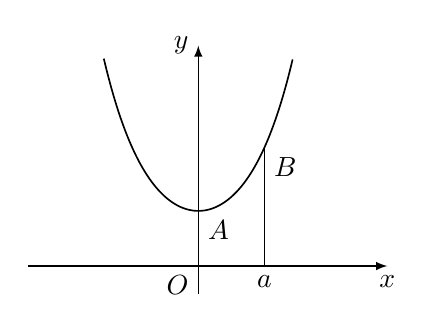
\begin{tikzpicture}[>=latex,xscale=1.2,yscale=0.7]
  \draw[->](-1.8,0)--(2.0,0)node[below]{$x$};
  \draw[->](0,-0.5)--(0,4.0)node[left]{$y$};
  \draw[semithick,samples=200,domain=-1:1]plot(\x,{0.5*(exp(2*\x)+exp(-2*\x))});
  \node at(0,1)[below right]{$A$};
  \node at(0,0)[below left]{$O$};
  \draw(0.7,{0.5*(exp(1.4)+exp(-1.4))})node[below right]{$B$}--(0.7,0)node[below]{$a$};
\end{tikzpicture}
\end{document}